\section{SQL-Parser}

\subsection{über den SQL-Parser: ZQL}

Auf der Webseite vom \cite{zql1} Projekt ist der Open-Source-Parser ZQL zu finden, welcher in der Lage ist SQL zu parsen und in Datenstrukturen zu überführen. Der Parser selbst ist mit \cite{javacc1} geschrieben, einem  Java-Parsergenerator (zu vergleichen mit dem populärem Unix yacc Generator).

ZQL bietet Unterstützung für \verb|SELECT-|, \verb|INSERT-|, \verb|DELETE-|, \verb|COMMIT-|, \verb|ROLLBACK-|, \verb|UPDATE-| und \verb|SET TRANSACTION-|Ausdrücke. Wichtig für diese Arbeit sind dabei insbesondere \verb|SELECT-| und \verb|UPDATE-|Ausdrücke, sowie -- die leider nicht enthaltenen -- \verb|CREATE TABLE-|Ausdrücke.

\subsection{Funktionsweise des Parsers}

ZQL kennt zwei grundlegende Interfaces \verb|ZExp| und \verb|ZStatement|. Wichtig für die weiterführende Erklärung ist, dass genau drei Klassen das Interface \verb|ZExp| implementieren. Diese werden im Folgenden auch vorgestellt. Es handelt sich um \verb|ZExpression, ZConstant, ZQuery|.

Das Interface \verb|ZStatement| bildet eine abstrakte Oberklasse für alle möglichen Arten von SQL-Statements. Folgende Klassen implementieren dieses Interface in ZQL:

\begin{itemize}
\item \verb|ZDelete| - repräsentiert ein \verb|DELETE| Statement
\item \verb|ZInsert| - repräsentiert ein \verb|INSERT| Statement
\item \verb|ZUpdate| - repräsentiert ein \verb|UPDATE| Statement
\item \verb|ZLockTable| - repräsentiert ein \verb|SQL LOCK TABLE| Statement
\item \verb|ZQuery| - repräsentiert ein \verb|SELECT| Statement
\end{itemize}

Das Interface \verb|ZExp| bildet eine abstrakte Oberklasse für drei verschiedene Arten von Ausdrücken:

\begin{itemize}
\item \verb|ZConstant| - Konstanten vom Typ \verb|COLUMNAME, NULL, NUMBER, STRING| oder \verb|UNKNOWN|
\item \verb|ZExpression| - Ein SQL-Ausdruck bestehend aus einem Operator und einen oder mehreren Operanden
\item \verb|ZQuery| - Eine \verb|SELECT| Anfrage ist auch ein Ausdruck
\end{itemize}

Wir klären in diesem Abschnitt nun genauer, wie der Parser SQL-Anfragen in interne Datenstrukturen überführt.
Dazu müssen die Datentypen des Parserpaketes zunächst erläutert werden. Anschließend stellen wir eine Beispielanfrage und ihre Überführung in die Datenstrukturen des Parsers vor. Daraus leiten wir auch die Schwächen bzw. Grenzen des Parsers ab. Wir stellen im Folgenden dar, was für relevante Attribute und Methoden die jeweiligen Klassen besitzen. Da viele Klassen durch Vererbung entstehen, werden wir der Übersicht halber auch abgeleitete relevante Attribute und Funktionen mit einbeziehen.

Die Klasse \textbf{ZFromItem} bezeichnet genau eine Tabelle. Gespeichert wird in dieser Klasse daher der \textit{Name der Tabelle} und ein möglicher \textit{Alias}.

Ähnlich ist die Klasse \textbf{ZSelectItem} aufgebaut. Sie speichert den Namen des Attributs und einen eventuell angegebene Tupelvariable. Weiterhin wird festgehalten, ob das SelectItem ein Ausdruck ist wie \mbox{z. B.} in \verb|SELECT a+b|. In diesem Fall würde man über die Funktion \verb|getExpression()| ein Objekt einer Klasse erhalten, die von \verb|ZExp| erben muss. Weiterhin wird gespeichert, ob es sich um eine Wildcard \verb|*| handelt oder ob das Item eine Aggregatesfunktion ist. Bei \verb|SELECT AVG(sal) FROM ...| würde der Name des Items \verb|sal| sein und die Aggregatsfunktion ist dann \verb|AVG|. 

Der \verb|WHERE|-Teil wird dargestellt mit Hilfe der Klasse \textbf{ZExpression}. Diese Klasse implementiert das Interface \verb|ZExp|. Ein Objekt der Klasse \verb|ZExpression| besteht immer aus einem Operator und mehreren Operanden. Ein Operator ist ein gültiger String. Was ZQL für gültige Operatoren kennt wird im Anhang aufgeführt. Ein Ausdruck speichert seine Operanden als \textit{Vector} von Objekten, die das Interface \verb|ZExp| implementieren. Demnach kann ein Operand vom Typ \verb|ZExpression, ZConstant| oder \verb|ZQuery| sein.
Wichtig ist auch zu bemerken, dass ZQL nicht nur zwei Operanden pro Ausdruck kennt. 

Ein üblicher Syntaxbaum ist binär, wobei die Wurzel den Operator mit der höchsten Priorität darstellt. Alle Teilbäume sind als Ausdrücke zu verstehen, jeweils mit Operator als Wurzelknoten und Operanden als Kindknoten. Dabei kann ein Operand auch ein weiterer Ausdruck sein. Generell wird dabei das Prinzip der Assoziativität benutzt um \mbox{z. B.} für gleichrangige Operatoren eine Auswertungsreihenfolge festzulegen.

So würde der \verb|WHERE|-Teil von folgender SQL-Anfrage:
\begin{verbatim}
SELECT * FROM emp e WHERE e.sal > 1000 AND e.sal < 2000 AND e.id > 1234
\end{verbatim}

zu folgendem, geklammerten Ausdruck werden:
\begin{verbatim}
(((e.sal > 1000) AND (e.sal < 2000)) AND (e.id > 1234))
\end{verbatim}

\begin{figure}[h]
\label{baum1}
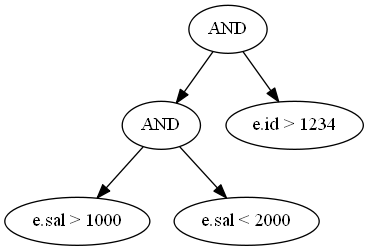
\includegraphics[scale=0.7]{Bilder/where_syntax.png}
\caption{WHERE-Bedingung in üblichen Syntaxbäumen}
\end{figure}

Der ZQL-Parser funktioniert so allerdings nicht. Wird keine spezielle Klammerung benutzt, so werden gleichrangige Operatoren nicht assoziativ geklammert, sondern befinden sich auf einer Ebene des Baumes. Somit handelt es sich nicht um einen binären Baum. 

Wir erhalten also aus obigen \verb|WHERE|-Ausdruck:
\begin{verbatim}
((e.sal > 1000) AND (e.sal < 2000) AND (e.id > 1234))
\end{verbatim}

\begin{figure}
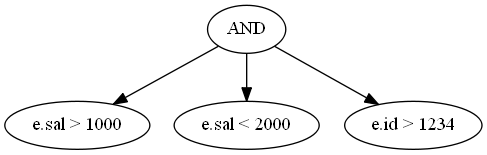
\includegraphics[scale=0.7]{Bilder/with_zql.png}
\caption{WHERE-Bedingung geparst mit ZQL}
\end{figure}
%ende baumerklaerung

So erklärt sich auch die Verwendung eines \textit{Vector} zur Speicherung der Operanden.

Die Klasse \textbf{ZConstant} dient zur Darstellung von SQL-Konstanten. Sie speichert den Wert der Konstante sowie den Typ. Als Typen kommen in Frage: \verb|COLUMNNAME, NULL, NUMBER, STRING, UNKNOWN|. Da die Typen selbsterklärend sind, wird auf eine detaillierte Beschreibung verzichtet.

Ein Objekt der Klasse \textbf{ZGroupBy} speichert im Wesentlichen zwei Informationen. Die \verb|GROUP BY| Ausdrücke werden gespeichert in einem \textit{Vector} von Klassen, die das \verb|ZExp| Interface implementiert haben. Der optionale \verb|HAVING BY| Ausdruck wird als Objekt einer der Klassen gespeichert, welche \verb|ZExp| implementieren. Typischerweise wird das ein Objekt der Klasse \verb|ZExpression| sein.

Die Klasse \textbf{ZOrderBy} speichert einzelne Sortierkriterien. Gebündelt werden diese dann über einen \textit{Vector}. Ein Objekt der Klasse \verb|ZOrderBy| enthält einen Ausdruck vom Typ \verb|ZExp| sowie die Information ob nach dem Suchkriterium aufsteigend oder absteigend sortiert werden soll.

Letztendlich vereinigt die Klasse \textbf{ZQuery} die eben vorgestellten Klassen. Die Funktion \verb|getSelect()| liefert einen \textit{Vector} von \verb|ZSelectItem| zurück. Ähnlich dazu liefert die Methode \verb|getFrom()| einen \textit{Vector} von \verb|ZFromItem| zurück. Hier erkennt man schon eine Beschränkung des Parsers. Da der \verb|FROM|-Teil nur als Ansammlung von \verb|FROM|-Items abstrahiert wird, werden Joins unter \verb|FROM| nicht vom Parser erfasst. Die Methode \verb|getWhere()| liefert ein Objekt zurück, was das Interface \verb|ZExp| implementiert haben muss. Typischerweise ist dies ein Objekt der Klasse \verb|ZExpression|. Analog dazu liefert die Methode \verb|getGroupBy()| ein Objekt der Klasse \verb|ZGroupBy| zurück. Die Methode \verb|getOrderBy| liefert einen \textit{Vector} von \verb|ZOrderBy|-Objekten zurück.
Schlussendlich existiert noch eine Methode \verb|isDistinct()|, die klärt ob ein \verb|DISTINCT| verwendet wurde.

Dies sind die am häufigsten gebrauchten Klassen des ZQL-Parser. Wir wollen nun die Arbeitsweise des Parsers anhand eines Beispieles verdeutlichen. Da die \verb|SELECT|-Anfragen die wohl am häufigsten gebrauchte Form der Anfragen ist, wird sich die Erklärung der Funktionsweise des Parsers beispielhaft auf diese Art der Anfragen beziehen. Wie die anderen Statements geparst werden ist dann analog schnell zu verstehen.


Eine gewöhnliches Select-Statement wird wie folgt vom Parser zerlegt:
\begin{verbatim}
SELECT e.name, sal, dname 
FROM emp e, dept d 
WHERE e.sal > 1000 AND e.did = d.id 
ORDER BY e.sal DESC\end{verbatim}

Die ganze Anfrage wird in einem Objekt vom Typ \verb|ZQuery| eingebettet. Wir gehen nun nacheinander die Bestandteile dieses Objektes durch. Wir schreiben vereinfacht eine Art Pseudocode. Elemente in einem Array oder Vector werden einfach als Menge \verb|{elem1, elem2, elem3}| dargestellt. Objekte werden vereinfacht dargestellt als Ansammlung von Attributen. Dies ist legitim, da die Methoden fast ausschließlich nur getter und setter sind. Ein Objekt o mit dem Attribut ``name'' und den Wert ``Otto'' schreiben wir daher als: 
\verb|o = { [name=Otto] }|

Der \textbf{SELECT}-Teil wird durch einen \textit{Vector} dargestellt. Alle Items sind vom Typ \textit{ZSelectItem}. \verb|SelectVector = { selItem1, selItem2, selItem3 }|.

\verb|selItem1 = { [Table=e], [Column=name], [Expression=false], [Wildcard=false] }|

\verb|selItem2 = { [Table=null], [Column=sal], [Expression=false], [Wildcard=false] }|

\verb|selItem3 = { [Table=null], [Column=dname], [Expression=false], [Wildcard=false] }|

Auch im \verb|FROM|-Teil finden wir einen \textit{Vector}, der nun aus Objekten vom Typ \verb|ZFromItem| besteht. \verb|FromVector = { fromItem1, fromItem2 }|.

\verb|fromItem1 = { [Table=emp], [Alias=e] }|
\verb|fromItem2 = { [Table=dept], [Alias=d] }|

Kommen wir nun zum komplexeren Teil, dem \verb|WHERE|-Ausdruck. Da diese Struktur baumartig ist, lässt sich dies zunächst besser in einem Bild ausdrücken.

\begin{figure}[h]
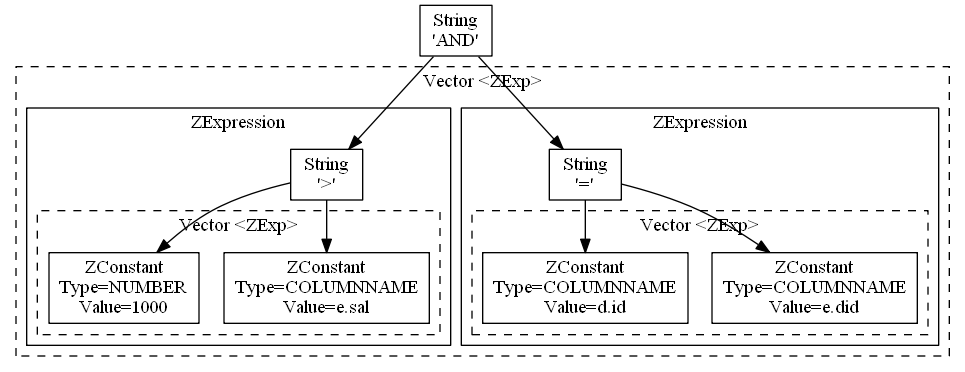
\includegraphics[scale=0.51]{Bilder/parserbaum.png}
\caption{Geparster Baum der WHERE Bedingung des Beispiels}
\label{fig:parseTree}
\end{figure}

In Abbildung \ref{fig:parseTree} sieht man nun den geparsten Baum der \verb|WHERE|-Bedingung. Die gestrichelten K"asten sollen andeuten, dass es sich um den \textit{Vector} von Klassen handelt, die \verb|ZExp| implementieren, während durchgezogene Kasten konkrete Objekte sein sollen.

\subsection{Grenzen des Parsers}
\label{subsec:grenzenparser}

Der Parser kann keine \verb|CREATE TABLE|-Statements parsen. Somit ist es im Rahmen dieser Arbeit notwendig, den Parser zu erweitern, damit Tabellen in eigene Datenstrukturen geparst werden können. Für die Arbeit ist es zunächst nur notwendig Name und Datentyp der Spalten in eine interne Datenstruktur zu überführen. Dabei wird nur zwischen Zahlen und Sonstigem (Text) unterschieden. Unser Programm soll in der Lage sein, einfache arithmetische Operationen durchzuführen. Dazu ist das wissen um Datentypen der Variablen von Nöten.

Weiterhin ist der ZQL-Parser nicht in der Lage \verb|JOINS| über die Schlüsselworte \\\verb#ON [LEFT OUTER|RIGHT OUTER|INNER] JOIN# zu realisieren. Der Parser erkennt nur innere \verb|JOINS|, die im \verb|WHERE|-Teil formuliert worden. Das soll für diese Arbeit ohne weitere Bedeutung sein, da dennoch Strategien entwickelt werden, wie man mit derartigen \verb|JOINS| umgeht. Es muss an der Stelle nur erwähnt werden, dass das Programm, welches im Rahmen dieser Arbeit entsteht, mit derartigen \verb|JOINS| nicht umgehen kann.

Trotz dieser Einschränkungen sind alle Konzepte, die in dieser Arbeit vorgestellt werden einfach auf jedweden SQL-Parser übertragbar.

%TODO: CREATE TABLE

\section{Java Server Pages}

\subsection{Überblick}

\subsection{Einbettung in JSP}

\subsection{Log}